\documentclass{article}

\usepackage[tmargin=0.5in,bmargin=0.25in]{geometry}
\usepackage{amsmath, amssymb, amsthm}
\usepackage{enumitem}
\usepackage{graphicx}
\usepackage{multicol}
\graphicspath{{./}}

\title{\vspace{-4ex}Math 341 Homework 8}
\author{Isaac Boaz}

\renewcommand{\arraystretch}{1.2}
\newcommand{\ceil}[1]{\lceil {#1} \rceil}

\begin{document}
\maketitle

\pagebreak

\section*{Problem 7}
\begin{enumerate}[label=(\alph*)]
    \item \begin{align*}
              \alpha = 1 - 0.9 & = 0.1  \\
              \alpha/2         & = 0.05
          \end{align*}
          \begin{align*}
              t_{\alpha, n-1} & = t_{0.05, 42}                        \\
                              & = \text{qt}(0.05,\ 42,\ \text{FALSE}) \\
                              & = 1.681952
          \end{align*}
          \begin{align*}
              \bar{x} & \pm t_{\alpha, n-1} \frac{s}{\sqrt{n}}             \\
                      & = 43698770 \pm 1.681952 \frac{40268914}{\sqrt{43}} \\
                      & = 43698770 \pm 10328788.03                         \\
                      & = [33369981.97, 54027558.03]
          \end{align*}
    \item
          \setlength{\columnsep}{-1.6in}
          \begin{multicols}{2}
              A rough distribution for this data would be an exponential distribution, as the sales seem to go from high at the beginning and fall off exponentially as time passes.
              Since the exponential distribution only has one parameter (\(\lambda\)), we know it can be reasonably estimated by its mean (\(\lambda \approx \mu = 43698770\)).
              \columnbreak
              \rightline{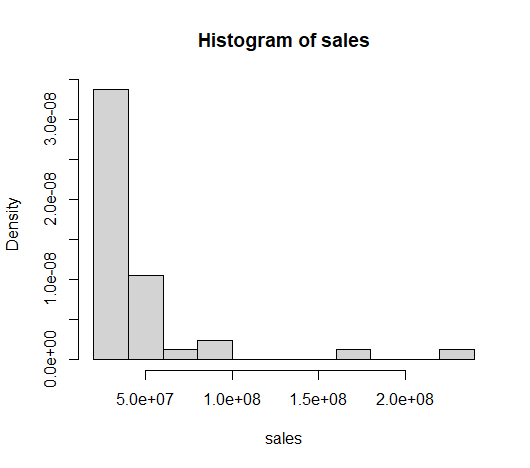
\includegraphics[width=0.3\textwidth]{histogram.png}}
          \end{multicols}
    \item Our estimation of \(\mu\) is most reliable when the random variables are normally distributed and independent. Since our dataset is clearly not normally distributed, it would require significantly more data samples (\(n \rightarrow 100+\)) to be able to estimate \(\mu\) with a high degree of confidence.
    \item \begin{align*}
              \bar{x}_1 - \bar{x}_1 \pm t_{\alpha/2,n_1+n_2-2} s_p \sqrt{1/n_1 + 1/n_2} \\
              s_p^2 = \frac{(n_1-1)s_1^2+(n_2-1)s_2^2}{n_1+n_2-2}
          \end{align*}
          \begin{align*}
              \bar{x}_1 = 52261232 & , n_1 = 22       \\
              \bar{x}_2 = 34728571 & , n_2 = 21       \\
              s_1 = 53743145       & , s_2 = 14403208
          \end{align*}
          \begin{align*}
              s_p^2 & = (\frac{(22 - 1) 53743145^2 + (21 - 1) 14403208^2}{22 + 21 - 2}) \\
                    & = \frac{64803886338136805}{41}                                    \\
          \end{align*}
          \begin{align*}
              52261232 - 34728571 & \pm t_{1-0.90, 22+21-2} \sqrt{\frac{64803886338136805}{41}} \sqrt{1/22 + 1/21} \\
              17532661            & \pm 1.682877946 \cdot 1.2128912 \times 10^7                                    \\
              17532661            & \pm 20411478                                                                   \\
                                  & [-2878817, 37944139]
          \end{align*}
    \item Since our interval contains 0, we can say there is not a significant difference between multi-platform vs. other games.
    \item It seems like the spreads are similar, so we can presumably trust the common variance assumption.
\end{enumerate}

\pagebreak
\section*{Problem 12}
\begin{enumerate}[label=(\alph*)]
    \item
          \begin{multicols}{2}
              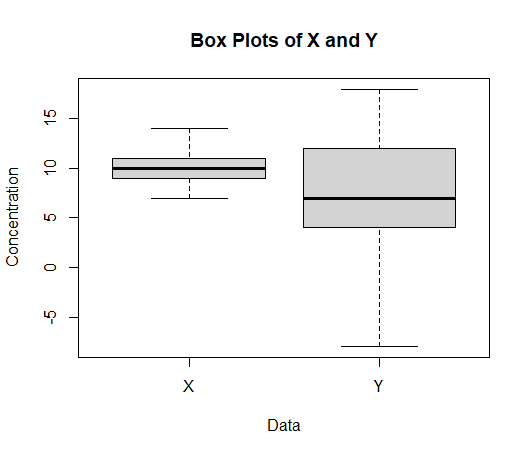
\includegraphics[width=0.45\textwidth]{xyboxplots.png} \\
              Looking at the boxplots, it seems like the \(Q_1\) and \(Q_3\)s are very different, implying that the variances (and thus standard deviations) are very different.
          \end{multicols}
    \item The generated histogram for x seems to be sufficiently symmetric, so we can assume that the distribution is normal.
          The generated histogram for y also seems to be sufficiently symmetric, with the majority of the samples occurring near the middle.
    \item Running a two-sample t-test (assuming common variance) on x and y we get a 95\% confidence interval of [-0.2183217, 5.1516550] with 48 degrees of freedom. Since this interval contains 0, we can say that there is no significant difference between the two samples.
    \item Running another two-sample t-test (not assuming common variance) on x and y we get a  95\% confidence interval of [0.1874896, 4.7458438] with 36.175 degrees of freedom. Since this interval does not contain 0, we can say there is a significant difference between the two samples.
\end{enumerate}

\pagebreak
\section*{Problem 13}
\begin{enumerate}[label=(\alph*)]
    \item Binomial Distrbution with \(n = 100\) and \(p = 0.05\) (success being a CI does not contain the mean \(\mu\)).
    \item \begin{align*}
              P(3 \leq\  & X < 8)                       \\
                         & = P(X \leq 7) - P(X < 3)     \\
                         & = P(X \leq 7) - P(X \leq 2)  \\
                         & \approx 0.872039 - 0.1182629 \\
                         & \approx 0.7537765
          \end{align*}
    \item \begin{align*}
              Poisson & \sim Bionmial    \\
              Y       & \sim Poisson(np) \\
                      & \sim Poisson(5)
          \end{align*}
          \begin{align*}
              P(3 \leq Y < 8) & = P(Y \leq 7) - P(Y < 3)    \\
                              & = P(Y \leq 7) - P(Y \leq 2) \\
                              & \approx 0.866628 - 0.124652 \\
                              & \approx 0.7419763
          \end{align*}
    \item The Poisson approximation is a good approximation for the binomial distribution when \(n\) is large and \(p\) is small, and the two probabilities reflect this.
\end{enumerate}
\pagebreak
\section*{Problem 14}
\begin{enumerate}[label=(\alph*)]
    \item To achieve a 95\% confidence interval with a margin of error being at most 0.025:
          \begin{align*}
              n & = \frac{z_{a/2}^2 \sigma^2}{E^2} \\
              n & = \frac{z_{a/2}^2 p(1-p)}{E^2}
          \end{align*}
          \begin{align*}
              E                                                               & = 0.025         \\
              \alpha = 1 - 0.98                                               & = 0.02          \\
              Z_{\alpha/2}                                         = Z_{0.01} &                 \\
              \text{invNorm(0.01, 0, 1, RIGHT)}                               & =  2.326        \\
              P                                                               & \rightarrow 0.5
          \end{align*}
          \begin{align*}
              n \geq \frac{2.326^2 0.5(1 - 0.5)}{0.025^2} \\
              \geq \ceil{2164.1104} = 2165
          \end{align*}
    \item For the life of a light bulb that is normally with \(\sigma = 25\). To find a CI with 95\% and error \(\leq 2.5\):
          \begin{align*}
              E = 2.5                                      \\
              \alpha = 1 - 0.95 = 0.05                     \\
              Z_{\alpha/2} = Z_{0.025}                     \\
              = \text{invNorm(0.025, 0, 1, RIGHT)} = 1.959 \\
              n \geq \frac{1.959^2 \cdot 25^2}{2.5^2}      \\
              \geq \ceil{383.76} = 384\end{align*}
    \item Creating a 95\% CI with an error at most 0.05 assuming \(0.1 \leq p \leq 0.3\):
          \begin{align*}
              E = 0.05                                         \\
              \alpha = 1 - 0.95 = 0.05                         \\
              Z_{\alpha/2} = Z_{0.025}                         \\
              = \text{invNorm(0.025, 0, 1, RIGHT)} = 1.959     \\
              P \rightarrow 0.3                                \\
              n \geq \frac{1.959^2 \cdot 0.3(1 - 0.3)}{0.05^2} \\
              \geq \ceil{322.365204} = 323
          \end{align*}
\end{enumerate}

\end{document}